\chapter[The Generalized Lambda Distribution]{The Generalized Lambda Distribution}\label{cap:gld}

\begin{flushright}
	\textit{``There are good reasons for using the GLD distribution \\
	methods... GLD fits have been used successfully in many fields ...\\
	Try the GLD first and stop there if the results are acceptable.''\\
	(Karian and Dudewicz, 2011)}
\end{flushright}


Fitting statistical distribution to data (real or simulated) is an important task in uncertainty quantification forward problem. When fitting data, one typically first selects a general class, or family, of distributions and then finds values for the distributional parameters that best match the observed data \cite{Lakhany2000}. One of this families is the Generalized Lambda Distribution (\textit{GLD}), originally proposed by Ramberg and Schmeiser in 1974, as a generalization of the Tukey's distribution (1947). The \textit{GLD} has been used in for years to fit data in the most diverse areas such us: analysis of brain MRI scan data, human twin data for quantifying genetic (vs. environmental) variance, rainfall distributions, radiation in soil, velocities within galaxies, exchange rate data for Japanese yen, and so on \cite{Karian2011}. This is due to its flexibility to describe a variety of shapes and to provide good fits to many well known distributions.    

Contradictorily, the \textit{GLD} is not extensively used in UQ, despite the features that make it attractive for these purposes. In the present Chapter we show the features that motivated us to select the \textit{GLD} as a distribution to characterize the uncertainty in our proposed approach.

The rest of the Chapter is organized as follow: Section \ref{sec:parameterizations} presents the different parameterizations of the \textit{GLD}, highlighting the advantages and drawbacks of those parameterizations and justifying the selected one. In Section \ref{sec:gld_shapes} the shapes of the \textit{FMKL} parametrization of the \textit{GLD} are investigated. Next, in Section \ref{sec:gld_numerical_methods} the principal references to the numerical method to estimate the parameters of the \textit{GLD} are shown, with some considerations and comments about future works in this area. Section \ref{sec:gld_fit_other} shows how the \textit{GLD} fits many well know distributions. Section \ref{sec:gld_mixture} describes the flexibility of the \textit{GLD} to fit mixture of distributions (bimodal and multimodals). The ability of the \textit{GLD} as a random variate generator is presented in Section \ref{sec:gld_random_variate}, that reinforces the idea of using it in UQ context. In Section \ref{sec:gld_and_uq} we resume all the characteristics of the \textit{GLD} that makes it suitable to UQ. In Section \ref{sec:gldex} we present \textbf{GLDEX} an R package that represents the state-of-the-art of the algorithms to work with the \textit{GLD}. Finally in Section \ref{sec:gld_summary} we summarize the principal results of the Chapter.

\section{The Generalized Lambda Distribution}\label{sec:parameterizations}

The generalized lambda distribution is a continuous distribution defined in terms of its quantile function. Various parameterizations exist (see Section \ref{sec:gld_other_param}), but the most popular are the proposed by Ramberg and Schmeiser in 1974, Section \ref{sec:rs_gld}; and the proposed by Freimer et al. in 1988, Section \ref{sec:fmkl_gld}.

\subsection{The Ramberg and Schmeiser Parameterization}\label{sec:rs_gld}
The Generalized Lambda Distribution (\textit{GLD}) was proposed by Ramberg and Schmeiser in 1974 as an extention of the Tukey's distribution. It is represented by the quantil function:
\begin{equation}\label{eq:rs_param}
Q_{RS}(y|\lambda)=Q_{RS}(y|\lambda_{1}, \lambda_{2}, \lambda_{3}, \lambda_{4})=\lambda_{1}+\frac{y^{\lambda_{3}}-(1-y)^{\lambda_{4}}}{\lambda_{2}}
\end{equation}
where $Q_{RS}=F^{-1}$ is the quantile function for probabilities $y$, with $y\in[0,1]$; $\lambda_{1}$ and $\lambda_{2}$ are the location and scale parameters, and $\lambda_{3}$ and $\lambda_{4}$ determine the skewness and kurtosis of the $GLD(\lambda_{1}, \lambda_{2}, \lambda_{3}, \lambda_{4})$.

The probability density function of the \textit{GLD} at the point $x=Q_{RS}(y)$ is given by:
\begin{equation}\label{eq:rs_pdf}
f(x)=f(Q_{RS}(y))=\frac{\lambda_{2}}{\lambda_{3}y^{\lambda_{3}-1}+\lambda_{4}(1-y)^{\lambda_{4}-1}}
\end{equation}

In order to have a valid distribution function, the probability density function $f(x)$ need to be positive for all $x$ and integrates to one over the allowed domain:
\begin{equation}
f(x) \geqslant 0
\end{equation}
\begin{equation}
\int f(x)dx=1
\end{equation}

This imposes complex constraints on the parameters and support regions of the \textit{RS} parameterization, as summarized in table \ref{tab:rs_conts} and figure \ref{fig:rs_regions}.

% Please add the following required packages to your document preamble:
% \usepackage{multirow}
\begin{table}[]
\centering
\caption{Support regions of the GLD and conditions on the parameters given by the RS parameterization to define a valid distribution function \cite{Karian2011}. The support regions are displayed in Fig. \ref{fig:rs_regions}. Note that there are no conditions on $\lambda_{1}$ to obtain a valid distribution.}
\label{tab:rs_conts}
\begin{tabular}{c|c|c|c|c|c}
\hline
Region             & $\lambda_{2}$         & $\lambda_{3}$      & $\lambda_{4}$      & Q(0)                                                 & Q(1)                                                 \\ \hline
\multirow{3}{*}{1} & \multirow{3}{*}{$<0$} & $<=-1$             & $>=1$              & \multirow{3}{*}{$-\infty$}                           & \multirow{3}{*}{$\lambda_{1}+\frac{1}{\lambda_{2}}$} \\
                   &                       & $-1<\lambda_{3}<0$ & $>1$               &                                                      &                                                      \\
                   &                       & \multicolumn{2}{c|}{$\frac{(1-\lambda_{3})^{1-\lambda_{3}}(\lambda_{4}-1)^{\lambda_{4}-1}}{(\lambda_{4}-\lambda_{3})^{\lambda_{4}-\lambda_{3}}}=\frac{-\lambda_{3}}{\lambda_{3}}$}            &                                                      &                                                      \\ \hline
\multirow{3}{*}{2} & \multirow{3}{*}{$<0$} & $>=1$              & $<=-1$             & \multirow{3}{*}{$\lambda_{1}-\frac{1}{\lambda_{2}}$} &                                                      \\
                   &                       & $>1$               & $-1<\lambda_{4}<0$ &                                                      & $\infty$                                             \\
                   &                       & \multicolumn{2}{c|}{$\frac{(1-\lambda_{4})^{1-\lambda_{4}}(\lambda_{3}-1)^{\lambda_{3}-1}}{(\lambda_{3}-\lambda_{4})^{\lambda_{3}-\lambda_{4}}}=\frac{-\lambda_{4}}{\lambda_{3}}$}            &                                                      &                                                      \\ \hline
\multirow{3}{*}{3} & \multirow{3}{*}{$>0$} & $>0$               & $>0$               & $\lambda_{1}-\frac{1}{\lambda_{2}}$                  & $\lambda_{1}+\frac{1}{\lambda_{2}}$                  \\
                   &                       & $=0$               & $>0$               & $\lambda_{1}$                                        & $\lambda_{1}+\frac{1}{\lambda_{2}}$                  \\
                   &                       & $>0$               & $=0$               & $\lambda_{1}-\frac{1}{\lambda_{2}}$                  & $\lambda_{1}$                                        \\ \hline
\multirow{3}{*}{4} & \multirow{3}{*}{$<0$} & $<0$               & $<0$               & $-\infty$                                            & $\infty$                                             \\
                   &                       & $=0$               & $<0$               & $\lambda_{1}$                                        & $\infty$                                             \\
                   &                       & $<0$               & $=0$               & $-\infty$                                            & $\lambda_{1}$                                        \\ \hline
\end{tabular}
\end{table}

\begin{figure}[H]
    \centering
    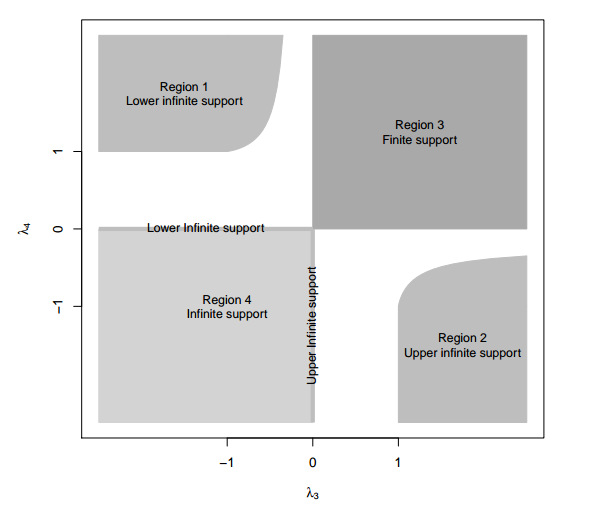
\includegraphics[width=0.8\textwidth]{img/gld/rs_regions.png}
    \caption{Support regions of the GLD in the RS parameterization that produce valid statistical
distributions.}
    \label{fig:rs_regions}
\end{figure}

\subsection{The FMKL Parameterization}\label{sec:fmkl_gld}
To circumvent the constraints on the \textit{RS} parameter values, Freimer et al. \cite{Freimer1988} introduced a new parameterization called \textit{FKML}, equation \ref{eq:fmkl_param}.

\begin{equation}\label{eq:fmkl_param}
Q_{FMKL}(y|\lambda_{1}, \lambda_{2}, \lambda_{3}, \lambda_{4})=\lambda_{1}+\frac{1}{\lambda_{2}}\left[\frac{y^{\lambda_{3}}-1}{\lambda_{3}} - \frac{(1-y)^{\lambda_{4}}-1}{\lambda_{4}} \right] 
\end{equation}

As in the previous parameterization, $\lambda_{1}$ and $\lambda_{2}$ are the location and scale parameters, but in this one $\lambda_{3}$ and $\lambda_{4}$ are the tail index parameters. The advantage over the previous parameterization is that the only constraint on the parameters is that $\lambda_{2}$ must be positive. Figure \ref{fig:fmkl_regions} displays the support regions of the \textit{GLD} in the \textit{FKML} parameterization, table \ref{tab:fmkl_conts}.

\begin{table}[H]
\centering
\caption{Support regions of the \textit{GLD} given by the \textit{FMKL} parameterization \cite{Marcondes2018}.}
\label{tab:fmkl_conts}
\begin{tabular}{c|c|c|c}
\hline
$\lambda_{3}$ & $\lambda_{4}$ & Q(0)                                           & Q(1)                                           \\ \hline
$>0$          & $>0$          & $\lambda_{1}-\frac{1}{\lambda_{2}\lambda_{3}}$ & $\lambda_{1}+\frac{1}{\lambda_{2}\lambda_{4}}$ \\ \hline
$>0$          & $\leq0$         & $\lambda_{1}-\frac{1}{\lambda_{2}\lambda_{3}}$ & $\infty$                                       \\ \hline
$\leq0$         & $>0$          & $-\infty$                                      & $\lambda_{1}+\frac{1}{\lambda_{2}\lambda_{4}}$ \\ \hline
$\leq0$         & $\leq0$         & $-\infty$                                      & $\infty$                                       \\ \hline
\end{tabular}
\end{table}

\begin{figure}[ht]
    \centering
    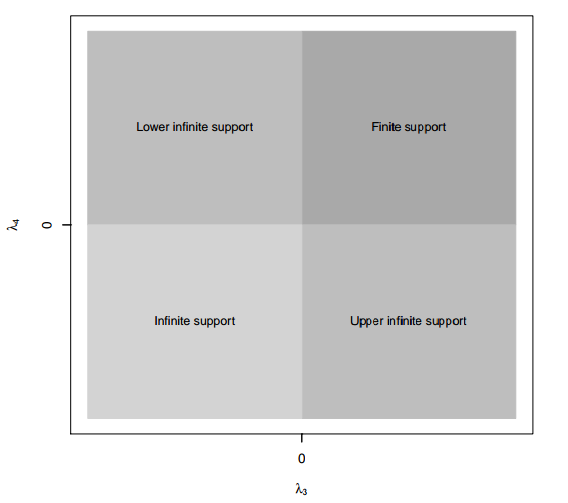
\includegraphics[width=0.8\textwidth]{img/gld/fmkl_regions.png}
    \caption{Support regions of the \textit{GLD} in the \textit{FMKL} parameterization that produce valid statistical
distributions.}
    \label{fig:fmkl_regions}
\end{figure}

The probability density function of the \textit{FMKL}-\textit{GLD} at the point $x=Q_{FMKL}(y)$ is given by \cite{Su2015}:
\begin{equation}\label{eq:fmkl_pdf}
f(x)=f(Q_{FMKL}(y))=\frac{\lambda_{2}}{y^{\lambda_{3}-1}+(1-y)^{\lambda_{4}-1}}
\end{equation}

Although both the \textit{RS} and \textit{FMKL} \textit{GLD} are generalizations of Tuckey's Lambda Distribution, they are not equivalent, so that the distribution fitted by one parametrization to a dataset differs in general from the one fitted by the other \cite{Marcondes2018}. Both of these representations can present a wide variety of shapes and therefore are utilized in practice; however, generally the \textit{FMKL GLD} is preferred due to the ease in its use \cite{Corlu2016}. In this thesis, we also use the \textit{FMKL GLD} representation.

\subsection{Other Parameterizations}\label{sec:gld_other_param}
One of the criticisms of the \textit{GLD} is that its skewness is expressed in terms of both tail indices $\lambda_{3}$ and $\lambda_{4}$. In one approach addressing this concern, a five-parameter \textit{GLD} was introduced by Joiner et al. \cite{Joiner1971}, which, expressed in the \textit{FKML} parameterization, can be written as,
\begin{equation}\label{eq:jr_param}
Q_{JR}(y|\lambda_{1}, \lambda_{2}, \lambda_{3}, \lambda_{4}, \lambda_{5})=\lambda_{1}+\frac{1}{2 \lambda_{2}}\left[(1-\lambda_{5})\frac{y^{\lambda_{3}}-1}{\lambda_{3}} - (1+\lambda_{5})\frac{(1-y)^{\lambda_{4}}-1}{\lambda_{4}} \right] 
\end{equation}

It has $\lambda_{1}$ and $\lambda_{2}$ as the location and scale parameters, and an asymmetry parameter, $\lambda_{5}$, which weights each side of the distribution and the two tail indices, $\lambda_{3}$ and $\lambda_{4}$. The conditions on the parameters are $\lambda_{2} > 0$ and $-1 < \lambda_{5} < 1$. The drawback of this parameterization is that the additional parameter can make the estimation of the parameter values even more difficult.

In \cite{Chalabi2012} the authors introduce a new parameterization of the \textit{GLD} that transforms the \textit{FMKL} parameterization, equation \ref{eq:fmkl_param} in terms of an asymmetry and steepness parameter without adding a new variable. Its major advantage is that it provides an intuitive interpretation of its parameters. A new \textbf{R} package called \textbf{gldist} was implemented with the new \textit{GLD} parameterization, along with the parameter estimation methods they present in their work. The problem with this parameterization is  that the \textbf{R} package was removed from the official repository because the code is out of date.

\section{FMKL GLD Shapes}\label{sec:gld_shapes}
Both \textit{RS} and \textit{FMKL} \textit{GLD} can describe a variety of shapes, such as: U-shaped, bell shaped, triangular, and exponentially \cite{Su2007}. At the same time they also provide good fits to many well know distributions. In the case of \textit{RS GLD} an extensive study can be found in \cite{Karian2011}, for the \textit{FMKL GLD} see \cite{Freimer1988}. 

Those properties of the \textit{GLD} are important to our purpose for two reasons: first we don't need previous knowledge to use the \textit{GLD} to fit any dataset, that is exactly the case in large-scale spatio-temporal models, and second the \textit{GLD} can be compared and grouped based on its shapes, that allows us to answer \textbf{RQ1} as we show in Chapter \ref{cap:gld_clustering}.

As the \textit{FMKL GLD} parameterization is the one selected to be used in this thesis, in the next sub-sections we present a brief review of its shapes and how this parameterization fits some well-known distributions.

The shape of the \textit{GLD} are dependent on its $\lambda$ values. In the case of the \textit{FMKL GLD} parameterization, Freimer et al. \cite{Freimer1988} classify the shapes into five categories depending on the variety of distributions that can be represented by the several combinations of the shape parameters $\lambda_{3}$ and $\lambda_{4}$. In particular, Class-I ($\lambda_{3} < 1$, $\lambda_{4}<1$) represents unimodal densities with continuous tails. This class is subdivided in $I_{a}$ $(\lambda_{3}, \lambda_{4} \leq 1/2)$, $I_{b}$ $(1/2 < \lambda_{3} < 1, \lambda_{4} \leq 1/2)$ and $I_{c}$ $(1/2 < \lambda_{3} < 1, 1/2 < \lambda_{4} < 1)$. In $I_{a}$ we find distributions such us $Gaussian (Normal)$, $Beta(2.3)$ and $\Gamma(\alpha = 5)$; in $I_{b}$ $\Gamma(\alpha = 3)$ and $Lognormal(\sigma=0.5)$; and in $I_{c}$ distributions as the example of Class-I in Figure \ref{fig:fmkl_classes}.  

Class-II ($\lambda_{3}>1$, $\lambda_{4}<1$) represents monotone pdfs similar to the $Exponential$ distribution, $Beta(1.2)$ or $Lognormal(\sigma=1.0)$. Class-III ($1<\lambda_{3}<2$, $1<\lambda_{4}<2$) represents U-shaped densities with truncated tails, Class-IV ($\lambda_{3}>2$, $1<\lambda_{4}<2$) represents S-shaped densities, and Class-V ($\lambda_{3}>2$, $\lambda_{4}>2$) represents unimodal densities with truncated tails. Figure \ref{fig:fmkl_classes} provides the shapes that are represented by the parameters indicated in Table \ref{tab:fmkl_classes}.

\begin{table}[H]
\centering
\caption{Examples of the five categories of distributions the \textit{FMKL GLD} can represent.}
\label{tab:fmkl_classes}
\begin{tabular}{lllll}
\hline
          & $\lambda_{1}$ & $\lambda_{2}$ & $\lambda_{3}$ & $\lambda_{4}$ \\ \hline
Class-I   & 0             & 1             & 0.5           & 0.6           \\
Class-II  & 0             & 1             & 2             & 0.5           \\
Class-III & 0             & 1             & 1.5           & 1.5           \\
Class-IV  & 0             & 1             & 2.5           & 1.5           \\
Class-V   & 0             & 1             & 3             & 3             \\ \hline
\end{tabular}
\end{table}

\begin{figure}[H]
    \centering
    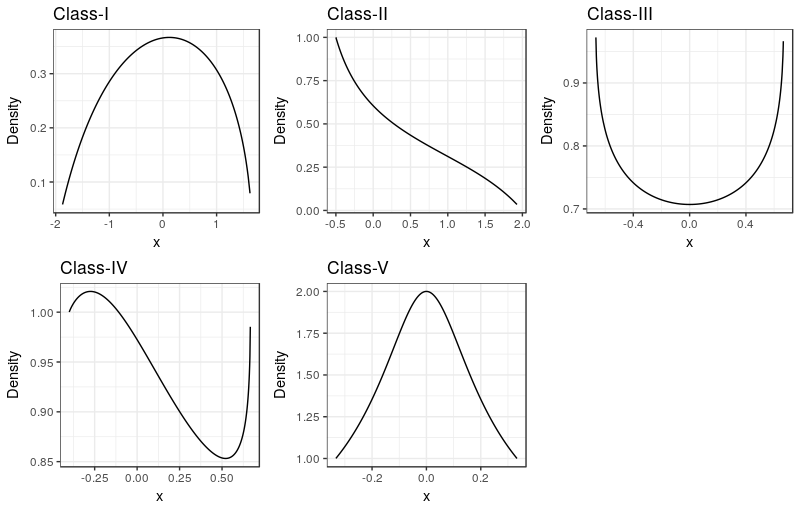
\includegraphics[width=0.8\textwidth]{img/gld/fmkl_classes.png}
    \caption{Examples of the five categories of shapes the \textit{FMKL GLD} can represent.}
    \label{fig:fmkl_classes}
\end{figure}

Figure \ref{fig:fmkl_classes_l3_l4} shows the five categories of the \textit{FMKL GLD} shapes in $(\lambda_{3}, \lambda_{4})$ space. There are two regions in this figure that were left out of the analysis, the regions with ($\lambda_{3}<1$, $\lambda_{4}>1$) and ($1<\lambda_{3}<2$, $\lambda_{4}>2$). Those regions are symmetric to region II and IV respectively, see Figure \ref{fig:symmetry}.

\begin{figure}[H]
    \centering
    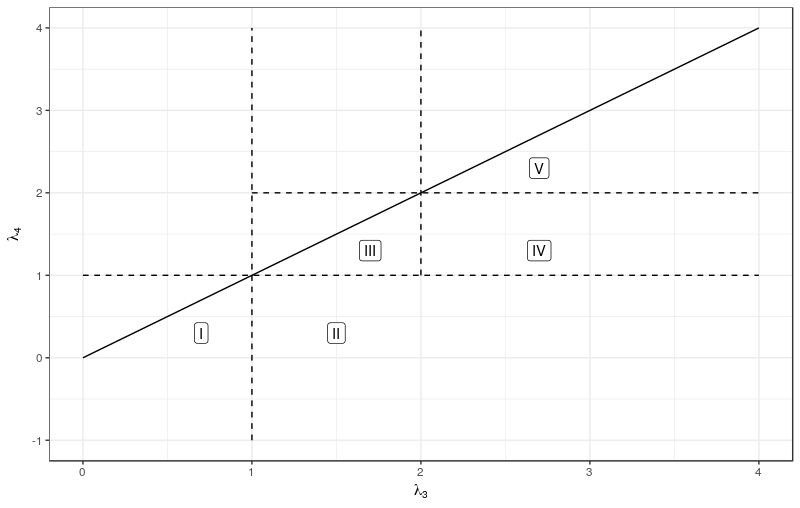
\includegraphics[width=0.8\textwidth]{img/gld/classes_l3_l4.png}
    \caption{The five categories of shapes of the \textit{FMKL GLD} in the $(\lambda_{3}, \lambda_{4})$ space.}
    \label{fig:fmkl_classes_l3_l4}
\end{figure}

\begin{figure}[H]
    \centering
    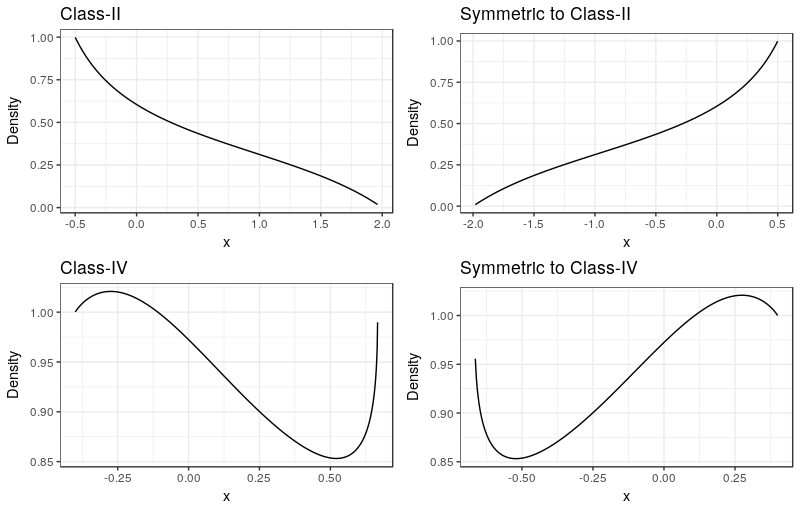
\includegraphics[width=0.8\textwidth]{img/gld/symetrics.png}
    \caption{Symmetry of the regions ($\lambda_{3}<1$, $\lambda_{4}>1$) and ($1<\lambda_{3}<2$, $\lambda_{4}>2$) with respect to  region II and IV.}
    \label{fig:symmetry}
\end{figure}

The results presented in this section are extremely important to our approach because they are the basis for the clustering algorithms we propose in Chapter \ref{cap:gld_clustering}.


\section{Numerical Methods to Fit the GLD to Data}\label{sec:gld_numerical_methods}
Given a random sample $x_{1},x_{2},x_{3},...x_{n}$, the basic problem in fitting a statistical distribution to this data is that of approximating the distribution from which the sample was obtained. If it is known, because of theoretical considerations, that the distribution is of a certain type (e.g., a gamma distribution with unknown parameters), then through moment matching, or some other means, one can determine a specific distribution that fits the data. This, however, is generally not the case and, in the absence of any knowledge regarding the distribution, it makes sense to appeal to a flexible family of distributions and choose a specific member of that family \cite{Karian2011}.

There are two different parameter estimation philosophies, \textbf{direct estimation methods}, such as least-squares estimation with order statistics and with percentiles \cite{Fournier2007, Karian2011}; the methods of moments \cite{Lodziensis2013}, L-moments \cite{Karvanen2008}, and trimmed L-moments \cite{Fournier2007}; and the goodness-of-fit method with histograms \cite{Su2005} and with maximum likelihood estimation \cite{Su2007}. On the other side, \textbf{stochastic methods} have been introduced with various estimators such as goodness-of-fit \cite{Lakhany2000} or the starship method [King and MacGillivray, 1999]. 

Without doubts the major contributions in the implementation of parameter estimation algorithms are due to Steve Su \cite{Su2007, Su2011, Su2015, Su2016}, that besides the theoretical contributions is the author of the state-of-the-art R package to work with the \textit{GLD}. A brief review of this package is presented in Section \ref{sec:gldex}, as this package is the one we use in this thesis to solve many task related to the \textit{GLD}.

Out of the two estimation philosophies presented above, \cite{Corlu2016} a genetic algorithms approach to estimate the parameters of the \textit{GLD} was introduced. 

Recently Marcondes at al. \cite{Marcondes2018} present a new parameterization of the \textit{GLD} with its respective numerical methods. The main contribution of this paper is that the new parameterization allows fitting the \textit{GLD} to highly skewed data, with a great number of zeros and heavy tails.

The methods to fit the \textit{GLD} to data are out of the scope of this thesis, as we are interested in demonstrating its usability in UQ. Nevertheless it is important to remark that, fit the \textit{GLD} to data is computationally intensive but suitable to parallelization, we haven't found any work in the literature to explore the possibility of increasing the performance of the fitting process by means of parallelization. This is an open problem we are interested in exploring in the future.    

\section{GLD Approximations of Some Well-Known Distributions}\label{sec:gld_fit_other}
For the $GLD(\lambda_{1}, \lambda_{2}, \lambda_{3}, \lambda_{4})$ to be useful for fitting distributions to data, it should be able to provide good fits to many distributions. In \cite{Karian2011}, the authors explore how the \textit{GLD} fit sixteen well-known distributions using the \textit{RS GLD} parameterization. Here we explore how the \textit{GLD} fit eight distributions, but using the \textit{FMKL} parameterization.

In Table \ref{tab:gld_fit_other} we show the original distribution, the four $\lambda$ values of the fit and the result of applying a Kolmogorov-Smirnov test to validate the good of the fit.

\begin{table}[H]
\centering
\caption{GLD Approximations of 8 Well-Known Distributions}
\label{tab:gld_fit_other}
\begin{tabular}{l|l|l|l|l|l|l}
\hline
Distribution & Parameters                    & $\lambda_{1}$ & $\lambda_{2}$ & $\lambda_{3}$ & $\lambda_{4}$ & KS-test \\ \hline
Normal       & $\textsc{N}(0, 1)$                     & -0.04263   & 1.49039    & 0.13787    & 0.12571    & 951     \\ \hline
Uniform      & $U(0, 1)$                     & 0.46250     & 2.16223     & 1.00008     & 0.8614     & 912     \\ \hline
Exponential  & $\theta = 1$                  & 0.49150     & 1.40546     & 1.44813     & -0.10419    & 923     \\ \hline
Chi-Square   & $nu = 5$                      & 4.141853    & 0.486702    & 0.508298    & -0.045440   & 911     \\ \hline
Gamma        & $(\alpha = 5, \theta = 3)$    & 1.535078    & 1.846312    & 0.410183    & 0.027492    & 885     \\ \hline
Weibull      & $(\alpha = 1, \beta = 5)$     & 2.684657    & 0.263865    & 1.413826    & -0.067658   & 940     \\ \hline
Lognormal    & $(\mu = 0, \sigma = 1/3)$     & 0.984696    & 4.516254    & 0.324879    & -0.074348   & 903     \\ \hline
Beta         & $(\beta_{3} = \beta_{4} = 1)$ & 0.50092     & 2.00702     & 0.99505     & 1.00060     & 906     \\ \hline
\end{tabular}
\end{table}

As expected the results are slightly different to those presented by Karian et al., as we use a different parameterization. The KS-test value was over 900 in seven cases and near 900 in the case of the Gamma distribution. This result suggests that the fit was good. All fits provide $(\lambda_{3}, \lambda_{4})$ values that match the shape region each distribution belongs to.


\section{Fitting Mixture Distributions Using a Mixture of Generalized Lambda Distributions}\label{sec:gld_mixture}
In general, a \textit{mixture distribution} is the probability distribution of a random variable that is derived from a collection of other random variables. Mathematically, given a finite set of \textit{PDFs} $p_{1}(x),p_{2}(x),\ldots,p_{n}(x)$, and weights $w_{1},w_{2},\ldots,w_{n}$ such that $w_{i} \geq 0$ and $\sum w_{i}=1$, the mixture distribution can be represented by writing the density $f(x)$ as a sum (which is a convex combination):

\begin{equation}
f(x)=\sum_{i}^n w_{i}p_{i}(x)
\end{equation}

Since its introduction by Karl Pearson in 1894 \textit{mixture distribution} are extensively used, but in the majority of the cases using normal mixtures. The advantage of using the \textit{GLD} family is that the \textit{GLD} can fit the normal distribution well. Hence whenever a mixture of normals would fit data well, so would a mixture of at most the same number of \textit{GLDs}. Meanwhile, the \textit{GLD} family is a much broader family, and can do well in cases where the normal cannot \cite{Ning2008}. Due to the versatile and rich shapes of the \textit{GLD}, they are particularly suited for mixture modeling as they eliminate the need to choose between a wide range of different distributions on the same data set \cite{Su2007}.

The \textit{GLD} mixture distribution can be represented as:
\begin{equation}
f(x)=\sum_{i}^n w_{i}GLD_{i}(\lambda_{1},\lambda_{2},\lambda_{3},\lambda_{4})
\end{equation}

Some studies that compare the use of \textit{GLD} mixtures with normal mixtures are presented by Ning et al. \cite{Ning2008}, where the author shows that the mixture of \textit{GLDs} performs as well as the mixture of normal distributions, and sometimes even better. In \cite{Su2011} the author presents examples of fitting bimodal and trimodal data with mixture of \textit{GLDs}, again with excellent results. Numerical methods to fit mixture of \textit{GLDs} to data are discused in \cite{Su2007, Su2011}, while the implementations are part of the \textbf{GLDEX} R package \cite{Su2007}.

We return to \textit{GLD} mixtures in Chapter \ref{cap:our_approach}, where we present how to answer the \textbf{RQ.3} by the use of a mixture of \textit{GLDs}.

\section{GLD Random Variate Generation}\label{sec:gld_random_variate}
An important thing to take into account when we substitute the raw data produced as an output of a simulation process, by its \textit{PDF} is that the latter needs to allow us to reproduce the original data as close as possible. The outcome produced by a particular \textit{PDF} is known as random variate, its definition is:

\begin{defn} 
A \textbf{random variate} is a particular outcome of a random variable. The random variates which are other outcomes of the same random variable might have different values.
\end{defn}

Random variates are used on simulating processes driven by random influences. One of the important applications of the \textit{GLD} has been the generation of random variables for Monte Carlo studies \cite{Mustafa2016}.

This fact is justified by the following theorem, enunciated by Karian and Dudewicz (2010).

\begin{thm}
If $Q_{X}(y)$ is the percentile function of a random variable $X$, and $U$ is a uniform random variable
on $(0, 1)$ then $Q_{X}(U)$ has the same \textit{PDF} as does $X$.
\end{thm}

For a proof, also see p. 156 of Karian and Dudewicz (1999). The percentile function is not available in a closed (or easy-to-work-with) form for many of the most important distributions, such as the normal distribution. However, the GLD is (see sections \ref{sub:rs_gld} and \ref{sub:fmkl_gld}) defined by its p.f., which is a simple-to-calculate expression.

Thus, \textbf{r.v.s for a simulation study can easily be generated from any distribution that can be modeled by a GLD.}

\begin{exmp}
Suppose we have modeled an important \textbf{r.v.} by an approximate standard normal distribution $X$. We show in Section \ref{sec:gld_fit_other} that a close fit to the standard normal is available via the \textit{RS-GLD} with 
\begin{equation}
(\lambda_{1}, \lambda_{2}, \lambda_{3}, \lambda_{4}) = (0, 0.1975, 0.1349, 0.1349)
\end{equation}
and this \textit{GLD} has \textbf{p.f.} 
\begin{equation}
Q(y) = \frac{y^{0.1349}-(1-y)^{0.1349}}{0.1975}
\end{equation}
\end{exmp}

Thus, if $U_{1}, U_{2},...$ are independent uniform \textbf{r.v.s} on $(0, 1)$, then 
\begin{equation}\label{eq:random_variate}
Q(U_{1}), Q(U_{2}),...
\end{equation}
are independent and (approximately) $N(0, 1)$ \textbf{r.v.s} for the simulation study at hand.

This theorem means that, independently of the nature of the dataset (Normal, Exponential, etc.), when we fit a GLD to it, we can proceed similarly to the example above. That is, we just need to generate a stream of independent uniform \textbf{r.v.s} on $(0, 1)$, and then evaluate the equation \ref{eq:random_variate}. There are a number of good sources of independent uniform r.v.s on $(0, 1)$ \cite{Karian2011}. 

This is an important property of the \textit{GLD} that allows us to substitute the raw data by the four lambdas of the \textit{GLD} that best fit it (if the fit is a good one), with the warranty that if we need to go back, the \textit{GLD} would generate a good representation of the original data.

It is evident that the \textit{GLD} allows easy generation of random variables from every kind of distribution, because featuring an explicit and accessible $Q_{X}(y)$ reduces it to a uniform generation in $[0,1]$, \cite{Lampasi2006}.


\section{GLD and Uncertainty Quantification}\label{sec:gld_and_uq}
From the best of our knowledge, the first effor to use the \textit{GLD} in UQ is due to Lampasi et al. \cite{Lampasi2006} in the paper \textit{"Generalized Lambda Distribution for the Expression of Measurement Uncertainty"}. In this paper the authors argue why the \textit{GLD} is suitable for UQ, (i) how the use of the \textit{GLD} to represent the uncertainty both at the input and the output of the models does help to homogenize the information we are processing in UQ worflows, (ii) the \textit{GLD} allows easy generation of random variables from every kind of distribution (see Section \ref{sec:gld_random_variate}), (iii) the amount of data we need to store is extremely smaller than required by histograms or by the approximation presented in \cite{Jcgm2008}, as a \textit{GLD} is fully described by its four parameters, and (iv) how their introduction is practical and suitable for automatic and software procedures, as required by the industrial standards.

Later Cox et al. \cite{Cox2012} comment that as the \textit{GLD} is defined with respect to its quantile function, drawing random samples from the resulting model approximation is straightforward, and then its use is suitable because it is not always convenient to retain the among of values produced by MC simulations and use them subsequently. Then we can substitute the raw data generated in MCS by the \textit{GLDs} that represent this raw data.

A more general reference of the use of the \textit{GLD} in UQ is due to Hack et al. in \cite{da2012measurement}. They do a literature review about UQ and include the \textit{GLD} as a very interesting option to characterize the uncertainty.

In \cite{Movahedi2013}, a solution to determine the reliability of products using the \textit{GLD} is presented. The novelty here is because of the variability of distributions of the products they need a flexible distribution family that allows to fit those distributions without previous knowledge.

Finally, in \cite{Rajan2016} the authors present a benchmark test distributions for expanded uncertainty evaluation algorithms. Between many other distributions, the \textit{GLD} is included because of its potential use in UQ. 

\subsection{Relevance of GLD in Uncertainty Quantification}
The use of the \textit{GLD} to quantify the uncertainty is justified because: 
\begin{itemize}
\item the \textit{GLD} fits the \textit{PDF} of a wide variety of datasets, including those that follow distributions such as normal, uniform, Student's t, U-shaped, exponential, etc;
\item no prior knowledge is needed to fit the \textit{GLD} to a dataset, which is practical and suitable for automatic and software procedures;
\item the \textit{PDF} is completely characterized by the four parameters of the \textit{GLD}, which represents a reduction in the amount of data that must be stored for post-processing;
\item the shape of the \textit{GLD} is governed by its parameters, so the \textit{GLDs} can be grouped  based on their shapes, which is especially useful for further queries;
\item in cases where mixture of distributions are needed, \textit{GLD} mixtures could be a very good option; and
\item the \textit{GLD} allows easy generation of random variables from every kind of distribution.
\end{itemize}

\section{The GLDEX R package}\label{sec:gldex}
In the implementation of our approach, we use the \textbf{\textit{GLDEX}}\footnote{https://cran.r-project.org/web/packages/GLDEX/index.html} \textbf{\textit{R}} package \cite{Su2007}. The GLDEX R package provides fitting algorithms with two objectives: (i) to provide a smoothing device to fit distributions to data using the weight and unweighted discretised approach based on the bin width of the histogram; (ii)  to provide a definitive fit to the data set using the maximum likelihood estimation.

The GLDEX package also provides diagnostic tests to examine the quality of fit through the resample Kolmogorov-Smirnoff test, quantile plots and comparison of the mean, variance, skewness and kurtosis between the empirical data and the fitted distribution.

The GLDEX package is used in this thesis to: (i) fit the \textit{GLD} distribution to a dataset on each spatio-temporal location; (ii) examine the quality of the fit; (iii) sampling any spatio-temporal location based on its \textit{GLD}.

\section{Summary}\label{sec:gld_summary}
The main contribution of this Chapter is to summarize the relevance of \textit{GLD} in UQ. Besides that, we select the \textit{FMKL} parameterization as the one we use in this thesis, because it is more general than the \textit{RS-GLD}. The shapes of the \textit{FMKL-GLD}, the capacity to describe many well know distributions and the fact that \textit{GLD} mixtures outperform normal mixtures, allow us to conclude that the \textit{GLD} is a good candidate to be used in our approach. 

The \textit{GLD} also fits the five requirements enunciated in Section \ref{sec:uq_large_scale} of Chapter \ref{cap:background}, as the desirable characteristics of a flexible family, to be used in the quantification of uncertainty in \textbf{LSSTM}.

